\documentclass[aspectratio=169,11pt]{beamer}

% ============================================================
% SISMID 2026 -- Day 2, 11:00 session
% More novel data streams (S. Yang + C. Djorno)
% Human mobility (ground + air), weather, news alerts.
% Grounded in what the field already uses: GLEAM (Vespignani/MOBS)
% for mobility, Shaman et al. for weather/humidity, HealthMap /
% ProMED / GDELT for news. Hands-on angle: free, scrapable proxies
% for the licensed gold-standard sources.
% Compile: pdflatex more-novel-data-streams.tex  (run twice)
% ============================================================

\IfFileExists{beamerthememetropolis.sty}{
  \usetheme{metropolis}
  \metroset{progressbar=frametitle, sectionpage=progressbar, numbering=fraction}
}{
  \usetheme{Boadilla}
  \usecolortheme{seahorse}
  \setbeamertemplate{navigation symbols}{}
}

\usepackage[utf8]{inputenc}
\usepackage[T1]{fontenc}
\usepackage{tikz}
\usetikzlibrary{arrows.meta, positioning, fit, backgrounds, calc}
\usepackage{xcolor}
\usepackage{listings}

\definecolor{AccentA}{HTML}{2A6F97}
\definecolor{AccentB}{HTML}{C1666B}
\definecolor{AccentC}{HTML}{3B8A5B}
\setbeamercolor{frametitle}{bg=AccentA}
\setbeamercolor{progress bar}{fg=AccentB}

\definecolor{skbg}{rgb}{0.96,0.96,0.94}
\lstdefinestyle{prompt}{
  basicstyle=\ttfamily\scriptsize,
  backgroundcolor=\color{skbg},
  showstringspaces=false, breaklines=true,
  frame=single, framesep=4pt, columns=fullflexible, numbers=none,
}
\lstset{style=prompt}

\tikzset{
  cbox/.style={draw=AccentA, very thick, rounded corners, align=center,
    minimum height=1.0cm, inner sep=6pt, font=\small, fill=AccentA!6},
  sbox/.style={draw=AccentA, thick, rounded corners, align=center,
    minimum height=0.85cm, inner sep=4pt, font=\scriptsize, fill=AccentA!6},
  rbox/.style={draw=AccentB, thick, rounded corners, align=center,
    minimum height=0.85cm, inner sep=4pt, font=\scriptsize, fill=AccentB!8},
  gbox/.style={draw=AccentC, thick, rounded corners, align=center,
    minimum height=0.85cm, inner sep=4pt, font=\scriptsize, fill=AccentC!8},
  flow/.style={-{Stealth[length=3mm]}, very thick, draw=AccentB},
  flowq/.style={-{Stealth[length=2.4mm]}, thick, draw=AccentA!70},
}

\title{More Novel Data Streams}
\subtitle{Mobility, weather, and news, borrowing what the field already uses}
\author{Shihao Yang \quad\textbullet\quad Candice Djorno}
\institute{SISMID 2026 \textbullet\ Day 2, 11:00}
\date{July 21, 2026}

\begin{document}

\begin{frame}
  \titlepage
\end{frame}

\begin{frame}{A different question}
  The streams so far (search, Wikipedia, wastewater) mostly answer \textbf{``how much
  disease is here now?''} These three answer different questions:
  \begin{itemize}
    \item \textbf{Mobility}: where is it \emph{coming from}?
    \item \textbf{Weather}: what is \emph{driving} it?
    \item \textbf{News}: what is \emph{emerging} that has no data yet?
  \end{itemize}
  \vspace{0.3em}
  \begin{block}{Honest framing}
    These are streams other groups pioneered: \textbf{GLEAM} (Vespignani's lab) for
    mobility, \textbf{Shaman et al.} for weather, \textbf{HealthMap / ProMED} for news. We
    credit them, and we show how to reach \emph{free, scrapable} versions with an agent.
  \end{block}
\end{frame}

\begin{frame}{Roadmap}
  \tableofcontents
\end{frame}

% ===============================================================
\section{Human mobility}

\begin{frame}{Disease travels with people, not with distance}
  Epidemics spread along how people actually move. Big, well-connected places seed smaller
  ones (the gravity / metapopulation intuition behind flu spread).
  \begin{itemize}
    \item \textbf{Ground} movement (commuting) drives local, radial spread between nearby
          counties.
    \item \textbf{Air} travel drives long-range importation, seeding distant places.
  \end{itemize}
  \vspace{0.3em}
  \begin{center}
    \itshape So two questions: which neighbors will seed me next, and which far-off places
    import risk to me?
  \end{center}
\end{frame}

\begin{frame}{The gold standard: GLEAM (Vespignani / MOBS lab)}
  The most established mobility-driven epidemic model, and worth knowing by name.
  \begin{itemize}
    \item \textbf{Air travel:} the \textbf{OAG} and \textbf{IATA} databases, roughly 3,800
          airports and 4M+ connections.
    \item \textbf{Ground:} a \textbf{commuting} database from 40+ national statistics
          offices, 78,000+ regions, 5M+ connections, mapped with Voronoi cells around
          airports.
    \item \textbf{Population:} WorldPop / Gridded Population of the World.
  \end{itemize}
  \vspace{0.3em}
  \begin{alertblock}{The catch for a hands-on class}
    OAG, IATA, and SafeGraph are \textbf{licensed}. We cannot scrape them live. So we use
    \textbf{free proxies} and keep cached snapshots of the licensed ones.
  \end{alertblock}
\end{frame}

\begin{frame}{Meet the source: US Census commuting data (LODES)}
  Every year the Census links \textbf{where people live} to \textbf{where they work}, from
  employment records. It is free, it covers the whole United States, and it goes down to the
  neighbourhood.
  \begin{itemize}
    \item Think of it as: \emph{``how many people sleep in county A and work in county B?''}
    \item That is the commuting shed, and it is the ground truth for which neighbours you
          actually exchange people with every single day.
  \end{itemize}
  \begin{exampleblock}{Open and demo}
    \texttt{onthemap.ces.census.gov} \\
    A clickable map: pick a county, and watch the arrows showing where its workers come
    from. Raw files live at \texttt{lehd.ces.census.gov/data/}.
  \end{exampleblock}
\end{frame}

\begin{frame}[fragile]{Ground mobility you can actually scrape}
  \begin{itemize}
    \item \textbf{US Census LODES} (origin-destination commuting) is free and detailed: who
          lives where and works where, down to the census tract.
    \item \textbf{Google COVID-19 Community Mobility} (archived 2020--2022) and the \textbf{ODT
          Flow Explorer} are free downloads; \textbf{SafeGraph} is licensed, so cached.
  \end{itemize}
  \begin{block}{Prompt}
  \begin{lstlisting}
Using US Census LODES origin-destination data, for Fulton
County, GA, rank the counties that send the most commuters
in. Return the top 10 as a tidy table. These are the
neighbors whose outbreaks tend to reach us first.
  \end{lstlisting}
  \end{block}
\end{frame}

\begin{frame}{Meet the source: OpenFlights}
  A volunteer-built, openly published database of the world's \textbf{airports and airline
  routes}. Not passenger counts, but the \emph{wiring diagram} of global air travel.
  \begin{itemize}
    \item Think of it as: \emph{``which airports have a direct flight to mine, and where are
          they?''}
    \item That wiring is what turns a distant outbreak into a local case, which is the whole
          idea behind importation risk.
  \end{itemize}
  \begin{exampleblock}{Open and demo}
    \texttt{openflights.org} \\
    Search an airport and it draws every route on a world map. The underlying
    \texttt{routes.dat} and \texttt{airports.dat} are plain text files we read directly.
  \end{exampleblock}
\end{frame}

\begin{frame}[fragile]{Air mobility you can actually scrape}
  \begin{itemize}
    \item \textbf{OpenFlights} publishes a free, no-key table of airline routes: the
          \emph{structure} of air connectivity, a workable stand-in for OAG/IATA.
    \item \textbf{OpenSky Network} has real flight data (ADS-B), but its API now needs a
          free account and OAuth2 credentials (anonymous requests get a 403), so it is a
          take-home rather than an in-class pull.
    \item Cross-check which countries a place \textbf{exchanges} with using Wikipedia (a
          trick from our own planning), then reason about importation risk.
  \end{itemize}
  \begin{block}{Prompt}
  \begin{lstlisting}
Rank the countries that connect to Atlanta (ATL) as a
proxy for air-importation risk. Use the free OpenFlights
routes.dat + airports.dat (no key): count inbound routes
to ATL by origin airport, map each to its country, and
plot the top 10 excluding domestic.
  \end{lstlisting}
  \end{block}
\end{frame}

\begin{frame}{Asked for: Meta's AI for Good datasets}
  A participant asked whether we could work with Meta's AI for Good data. Mostly
  \textbf{yes}, because Meta publishes through the \textbf{Humanitarian Data Exchange}
  (HDX), which has a free, open API.
  \begin{center}
  \footnotesize
  \begin{tabular}{lll}
    \hline
    \textbf{Dataset} & \textbf{In class?} & \textbf{How} \\
    \hline
    Relative Wealth Index      & \textbf{yes} & free per-country CSVs on HDX \\
    Movement Distribution Maps & \textbf{yes} & free on HDX, CC BY, current to June 2026 \\
    Activity Space Maps        & not directly & not on HDX; Meta's own portal \\
    Points of Interest         & not directly & not on HDX under Meta \\
    \hline
  \end{tabular}
  \end{center}
  \vspace{0.2em}
  \begin{center}
    \itshape Two of the four are usable today, with no application. Details next slide.
  \end{center}
\end{frame}

\begin{frame}{Meet the source: Meta Data for Good (via HDX)}
  Meta turns its data into \textbf{aggregated, privacy-protected} public goods and gives them
  away through the humanitarian data portal the UN and NGOs use.
  \begin{itemize}
    \item \textbf{Relative Wealth Index}: how well-off each 2.4\,km square is. A useful
          \emph{confounder}: wealth shapes housing, water storage and care-seeking.
    \item \textbf{Movement Distribution}: how far people travel from home, by region and day.
          The behaviour channel disease travels through.
    \item \textbf{224 datasets} in total, including Social Connectedness and population
          density maps.
  \end{itemize}
  \begin{exampleblock}{Open and demo}
    \texttt{data.humdata.org/organization/meta} lists all 224, each with a Download button.
    Meta's own write-ups: \texttt{dataforgood.facebook.com}.
  \end{exampleblock}
\end{frame}

% ===============================================================
\section{Weather}

\begin{frame}{Weather as a modulator, not a case count}
  Weather does not count cases; it \textbf{shifts the conditions} for transmission.
  \begin{itemize}
    \item \textbf{Influenza:} \textbf{absolute humidity} is the dominant driver. Shaman et
          al. showed virus survival and transmission fall as absolute humidity rises, and
          built humidity-driven flu forecasts.
    \item \textbf{Vector-borne (dengue, Zika):} \textbf{temperature and rainfall} govern the
          mosquito life cycle, so they modulate outbreak timing and size.
  \end{itemize}
  \vspace{0.3em}
  \begin{center}
    \itshape Mauricio picks up the modeling of weather-as-modulator this afternoon; here we
    just get the data.
  \end{center}
\end{frame}

\begin{frame}{Meet the source: Open-Meteo}
  A free weather service built for programs rather than people: give it a latitude,
  longitude and date range, and it returns decades of daily weather. \textbf{No account, no
  key, no cost} for our use.
  \begin{itemize}
    \item Think of it as: \emph{``the weather history of any point on Earth, as a table.''}
    \item Behind it sits \textbf{ERA5}, the research-grade reanalysis that most
          humidity-and-flu papers use, at \texttt{cds.climate.copernicus.eu}.
  \end{itemize}
  \begin{exampleblock}{Open and demo}
    \texttt{open-meteo.com/en/docs/historical-weather-api} \\
    A live form: type a city, tick \emph{temperature} and \emph{dew point}, and it builds the
    exact web address that returns the data. Paste that link in a browser to see the numbers.
  \end{exampleblock}
\end{frame}

\begin{frame}[fragile]{Weather you can actually scrape}
  \begin{itemize}
    \item \textbf{Open-Meteo} gives free historical and forecast weather with \textbf{no
          key}: ideal for an agent.
    \item \textbf{ERA5} (Copernicus) is the research-grade reanalysis (temperature and dew
          point at 0.25 degrees) behind most humidity studies.
  \end{itemize}
  \begin{block}{Prompt}
  \begin{lstlisting}
Using the Open-Meteo historical API (no key), pull daily
temperature and dew point for Atlanta since 2016. Compute
weekly absolute humidity from them, and overlay it on flu
ED visits so I can see whether low humidity precedes flu
season.
  \end{lstlisting}
  \end{block}
\end{frame}

% ===============================================================
\section{News alerts}

\begin{frame}{News: catching what has no data yet}
  For a genuinely \textbf{emerging} outbreak, there is no search history and no wastewater
  site. The earliest signal is a report.
  \begin{itemize}
    \item \textbf{ProMED} (human-curated, since 1994) and \textbf{HealthMap} (news wires,
          RSS, ProMED, WHO, auto-parsed and geocoded) are the established event-based
          systems. ProMED flagged COVID roughly a day before official notification.
    \item These feed WHO's EIOS and are used by CDC and WHO.
  \end{itemize}
  \vspace{0.3em}
  \begin{center}
    \itshape This is also a stream in Mauricio and Kogan's multi-source COVID forecasting:
    searches + news alerts + GLEAM.
  \end{center}
\end{frame}

\begin{frame}{Meet the sources: four ways to watch the news}
  \begin{itemize}
    \item \textbf{HealthMap} reads news and official reports automatically and pins them on a
          world map. \texttt{healthmap.org}
    \item \textbf{ProMED} is the opposite: human experts posting curated outbreak reports
          since 1994. It flagged COVID about a day before the official notice.
          \texttt{promedmail.org}
    \item \textbf{GDELT} indexes world news in 100+ languages, free and \textbf{with no key}.
          That is why it is the one we scrape in class. \texttt{gdeltproject.org}
    \item \textbf{Media Cloud} is the scholars' tool: 200M+ stories in curated
          \emph{collections}, built for studying how a topic is covered. Needs a
          \textbf{free API key}. \texttt{search.mediacloud.org}
  \end{itemize}
  \begin{exampleblock}{Open and demo}
    \texttt{healthmap.org} (dots on a map), \texttt{promedmail.org} (one curated post), then
    \texttt{search.mediacloud.org} (attention over time by outlet).
  \end{exampleblock}
\end{frame}

\begin{frame}[fragile]{News you can actually scrape}
  \textbf{GDELT} monitors world news in 100+ languages, is 100\% free, and has an API,
  which makes it perfect for an agent. Or point the agent at a news filter directly.
  \begin{block}{Prompt}
  \begin{lstlisting}
Using the GDELT DOC 2.0 API, find news articles from the
past month that mention dengue outbreaks. Return date,
country, and headline; then summarize which countries are
newly reporting activity, as an emerging-outbreak watch.
  \end{lstlisting}
  \end{block}
  \begin{center}
    \itshape Noisy by nature: news reflects attention and reporting, so a human read is part
    of the loop.
  \end{center}
\end{frame}

% ===============================================================
\section{Social and survey signals}

\begin{frame}{What happened to Twitter and Facebook}
  The streams that powered 2020 research have mostly closed their doors.
  \begin{center}
  \footnotesize
  \begin{tabular}{lll}
    \hline
    \textbf{Source} & \textbf{Today} & \textbf{Why it matters} \\
    \hline
    X / Twitter posts      & paid API since 2023   & the classic firehose is gone \\
    Facebook posts         & CrowdTangle shut 2024 & research access by application only \\
    Bluesky                & \textbf{open}         & the workable social option \\
    Facebook symptom survey & \textbf{open} via CMU Delphi & the good part survived \\
    \hline
  \end{tabular}
  \end{center}
  \vspace{0.3em}
  \begin{alertblock}{The lesson worth remembering}
    Our own COVID exercise file still has \textbf{Twitter, Kinsa and Cuebiq} columns, and all
    three of those streams are now closed or gone. Novel data streams are \textbf{fragile};
    that is the argument for an agent that can re-scrape whatever exists today.
  \end{alertblock}
\end{frame}

\begin{frame}{Meet the source: Bluesky}
  A public social network with an \textbf{open door}: anyone can read public posts without an
  account, which is exactly what Twitter stopped allowing.
  \begin{itemize}
    \item Think of it as: \emph{``a Twitter-shaped network you are still allowed to read.''}
    \item One catch: \textbf{keyword search} needs a login, but \textbf{finding accounts} and
          \textbf{reading their public posts} does not. So we watch \emph{accounts}
          (epidemiologists, health agencies) rather than searching words.
  \end{itemize}
  \begin{exampleblock}{Open and demo}
    \texttt{bsky.app} \\
    Search \emph{dengue} or \emph{outbreak} in the website's own search box (the browser can
    do what the open API will not), then open a public-health account and scroll its feed.
    That feed is exactly what our notebook reads.
  \end{exampleblock}
\end{frame}

\begin{frame}{Meet the source: CMU Delphi (and the Facebook survey)}
  You cannot get Facebook \emph{posts}, but for two years Facebook asked millions of users
  \textbf{``is anyone in your household ill?''}, and Carnegie Mellon turned it into a public
  health signal.
  \begin{itemize}
    \item Think of it as: \emph{``a nationwide symptom survey, every day, free.''}
    \item It ships \textbf{error bars and sample sizes}, which almost no other novel stream
          does. It ran 2020 to June 2022: a benchmark, not a live feed.
  \end{itemize}
  \begin{exampleblock}{Open and demo}
    \texttt{delphi.cmu.edu/covidcast/survey-results} \\
    Delphi's \textbf{CTIS Dashboard}, for what they themselves call
    ``\emph{the Facebook Covid Survey}''. Signal definitions:
    \texttt{cmu-delphi.github.io/delphi-epidata}.
  \end{exampleblock}
\end{frame}

% ===============================================================
\section{Pulling it together}

\begin{frame}{The pattern behind all three}
  \begin{center}
  \resizebox{0.9\textwidth}{!}{%
  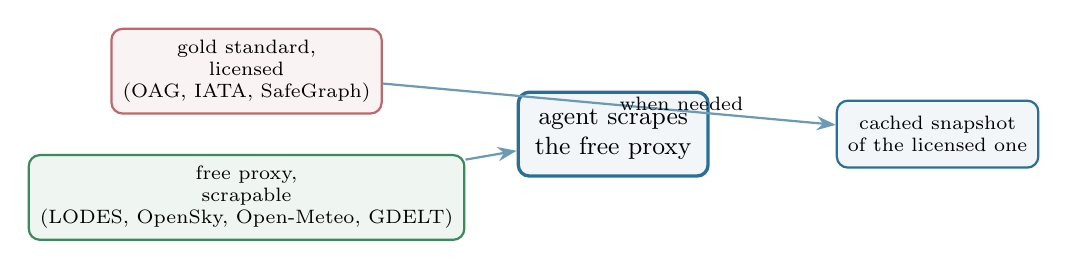
\begin{tikzpicture}[node distance=0.5cm and 1.2cm]
    \node[rbox] (lic) {gold standard,\\licensed\\(OAG, IATA, SafeGraph)};
    \node[gbox, below=of lic] (free) {free proxy,\\scrapable\\(LODES, OpenSky, Open-Meteo, GDELT)};
    \node[cbox, right=1.7cm of lic, yshift=-0.8cm] (a) {agent scrapes\\the free proxy};
    \node[sbox, right=1.6cm of a] (c) {cached snapshot\\of the licensed one};
    \draw[flowq] (free) -- (a);
    \draw[flowq] (lic) -- node[right,font=\scriptsize]{when needed} (c);
  \end{tikzpicture}}
  \end{center}
  \vspace{0.3em}
  \begin{itemize}
    \item Same five-step loop, same verify habit as every other stream.
    \item These are \textbf{context} signals (spread, drivers, emergence), noisier than a
          local case proxy. Treat them as complements, and validate.
  \end{itemize}
\end{frame}

\begin{frame}{Where this connects}
  \begin{itemize}
    \item \textbf{This afternoon:} the network / ARGONet idea borrows signal from neighbors,
          which is exactly what \textbf{ground mobility} tells you to do. Mauricio also covers
          \textbf{weather} and \textbf{news} for emerging outbreaks.
    \item \textbf{Day 3 capstone:} pick the streams that fit your question. Importation risk?
          Use air mobility. Seasonality? Weather. Emerging threat? News.
  \end{itemize}
  \vfill
  \begin{center}
    \itshape You now know the field's established streams by name, and a free, agent-scrapable
    way into each.
  \end{center}
\end{frame}

\begin{frame}{Credits and sources}
  \footnotesize
  \begin{itemize}
    \item \textbf{Mobility / GLEAM:} Balcan et al., \emph{Multiscale mobility networks and
          the spatial spreading of infectious diseases}, PNAS 2009; the GLEAM Project (MOBS
          lab, Northeastern; Vespignani). Data: OAG, IATA, national commuting statistics,
          WorldPop.
    \item \textbf{Free mobility proxies:} US Census LODES; OpenSky Network; Google COVID-19
          Community Mobility Reports (archived); ODT Flow Explorer.
    \item \textbf{Weather:} Shaman \& Kohn (PNAS 2009) and Shaman et al. (PLoS Biology 2010;
          PNAS 2012) on absolute humidity and influenza. Data: Open-Meteo; ERA5 (Copernicus).
    \item \textbf{News:} ProMED (ISID); HealthMap (Brownstein / Freifeld); WHO EIOS; GDELT.
          Multi-source forecasting: Kogan, Santillana et al., \emph{Science Advances} 2021.
  \end{itemize}
\end{frame}

\begin{frame}[standout]
  Questions?\\[0.4em]
  \small Repo: \texttt{github.com/Shihao-Yang/sismid2026}
\end{frame}

\end{document}
